\documentclass[11pt, oneside]{article}   	% use "amsart" instead of "article" for AMSLaTeX format
\usepackage{geometry}                		% See geometry.pdf to learn the layout options. There are lots.
\geometry{letterpaper}                   		% ... or a4paper or a5paper or ... 
%\geometry{landscape}                		% Activate for for rotated page geometry
%\usepackage[parfill]{parskip}    		% Activate to begin paragraphs with an empty line rather than an indent
\usepackage{graphicx}				% Use pdf, png, jpg, or eps� with pdflatex; use eps in DVI mode
								% TeX will automatically convert eps --> pdf in pdflatex		
\usepackage{amssymb}
\usepackage{amsmath}
\usepackage{parskip}

\graphicspath{{/Users/telliott_admin/Dropbox/Tex/png/}}

\title{Sphere sliced by a plane}
\date{}
\begin{document}
\maketitle
\Large

Start with the unit sphere centered at the origin.

\[ x^2 + y^2 + z^2 = 1 \]

Now, consider a plane which slices off a cap of the sphere, where the plane has normal vector

\[ \mathbf{n} = \ <0,1,1> \]

(the normal vector is orthogonal to the $x$-axis, which is parallel to the plane, and two points in the plane are $(0,1,0)$ and $(0,0,1)$.  The equation of the plane is

\[ \mathbf{n} \cdot <x,y, z> \  = d \]
\[ y + z = d \]

Plug in one of our points to find $d=1$ so
\[ y + z = 1 \]

How to find the volume of this region?  Much the easiest way is to rotate it so that the plane is parallel to the $xy$-plane and the region becomes symmetrical about the $z$-axis.  Then use cylindrical or spherical coordinates.  We just need to find the point $P$ which is on the plane and closest to the origin $O$, then compute the distance from $O$ to $P$.

\[ P = O + t<0,1,1> \ = (0,t,t) \]

P is in the plane so

\[ t + t = 1 \]
\[ P = (0,\frac{1}{2},\frac{1}{2}) \]

And the distance is then $1/\sqrt{2}$.

We could also do this part simply by looking at a cross-section in the $yz$-plane, considering the right triangle which includes the origin and our two points in the plane (on the $y$- and $z$-axes).  The sides of the triangle have length $1$ so the hypotenuse has length $\sqrt{2}$.  The coordinates of the midpoint of the hypotenuse are $(0,1/2,1/2)$ and the distance of the midpoint from the origin is $1/\sqrt{2}$.

\subsection*{General result by method of disks}

A method from single variable calculus to do this problem involves revolution of the unit circle.  I will change orientations (again) and revolve around the $x$-axis.  The function to use is the top half of a circle

\[ f(x) = + \sqrt{R^2 - x^2} \]

When we revolve a function $f(x)$ to generate a volume, the area of each "disk" is $\pi f(x)^2$, and adding them all up we obtain:

\[ V = \pi \int_a^b (R^2 - x^2) \ dx \]

We use constants $a$ and $b$ as the limits of integration with the understanding that $0 \le a < b  \le R$.

\[ = \pi \ ( \ R^2 x - \frac{x^3}{3} ) \ \bigg |_a^b  \]
\[ = \pi \ [ \ R^2 b - \frac{b^3}{3} - R^2 a +  \frac{a^3}{3} \ ] \]

For $a=0, b=R$, this becomes

\[ V = \pi \ [ \ R^3 - \frac{R^3}{3} - 0 +  0) = \frac{2}{3} \pi R^3 \ ] \]

as we expect for the semisphere.  

In this particular problem we have from above that $b=R=1$ so

\[ V = \pi \ [ \ R^2 b - \frac{b^3}{3} - R^2 a +  \frac{a^3}{3} \ ] \]
\[ V = \pi \ [ \ 1 - \frac{1}{3} - a +  \frac{a^3}{3} \ ] \]

and 

\[ a = \frac{1}{\sqrt{2}} \] 

giving 

\[ V = \pi \ [ \ \frac{2}{3} - \frac{1}{\sqrt{2}} +  \frac{1}{3} \ \frac{1}{2} \ \frac{1}{\sqrt{2}}\ ] \]
\[ V = \pi \ ( \frac{2}{3} - \frac{5}{6} \ \frac{1}{\sqrt{2}} ) \]

Our integration approach below will have a factor of $2 \pi/3$ out front so we'll do that here as well as well.

\begin{equation}
\boxed{ V = \frac{2}{3} \pi \ ( 1 - \frac{5}{4 \sqrt{2}} )}
\end{equation}

\subsection*{Wolfram formula for spherical cap}

The Wolfram formula uses different notation than what I've been using.  Here is their sketch:

\begin{center} 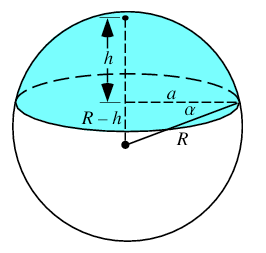
\includegraphics [scale=0.6] {spherical_cap.png} \end{center}

So first of all, they use $a$ for the radius of the circle where the plane intersects the sphere (which I call $r$ below and which doesn't even appear in my formula).  And then second, they write the formula in terms of $h$, the height of the cap, rather than the distance from the origin where the cap starts.

They give two formulas (I am using $r$ for the radius of the circle rather than $a$ as shown in the diagram)

\[ V = \frac{1}{6} \pi h (3r^2 + h^2) \]

and then an equivalent one which doesn't involve $r$:

\[ V = \frac{1}{3} \pi h^2 (3R - h) \]

What I'm going to do is first to start with our formula

\[ V = \pi \ [ \ R^2 b - \frac{b^3}{3} - R^2 a +  \frac{a^3}{3} \ ] \]

then setting $b=R$ we have

\[ V = \pi \ [ \ \frac{2}{3}R^3 - R^2 a +  \frac{a^3}{3} \ ] \]

Now, we will show that this is equivalent to the second Wolfram form, after substitution of $R-a$ for $h$.  Here goes:

\[ V = \frac{1}{3} \pi h^2 (3R - h) \]
\[ V = \frac{1}{3} \pi (R-a)^2 (3R - (R-a)) \]
\[ = \frac{1}{3} \pi (R^2 - 2Ra + a^2)(2R + a) \]
\[ = \frac{1}{3} \pi (2R^3 + R^2a - 4R^2a - 2Ra^2 + 2Ra^2 + a^3) \]
\[ = \frac{1}{3} \pi (2R^3 - 3R^2a + a^3) \]
\[ = \pi (\frac{2}{3}R^3 - R^2a + \frac{a^3}{3}) \]

and that's a match!

\subsection*{Using our write-up on spherical cap}

We have already looked at the formula for the volume of a spherical cap.

\[ V_{cap} = \frac{1}{3} \pi h^2(3R - h) \]

This is the same as Wolfram \#2.

In this particular problem, $R = 1$, so $h = 1 - a$, and the formula gives

\[ V_{cap} = \frac{1}{3} \pi \ [ \ (1-a)^2(3 - (1-a)) \ ] \]
\[ = \frac{1}{3} \pi \ (1 - 2a + a^2)(2 + a) \]
\[ = \frac{1}{3} \pi \ (2 + a - 4a - 2a^2 + 2a^2 + a^3) \]
\[ = \frac{1}{3} \pi \ (2 - 3a + a^3) \]
\[ = \frac{1}{3} \pi \ (2 - \frac{3}{\sqrt{2}} + \frac{1}{2 \sqrt{2}}) \]
\[ = \frac{1}{3} \pi \ (2 - \frac{5}{2\sqrt{2}} \]

Our answer in section one has a factor of $2/3$ out front so

\[ = \frac{2}{3} \pi \ (1 - \frac{5}{4\sqrt{2}} \]

That's a match!

We also have a formula for a spherical belt below the cap (which is just an adjustment of the limits of integration in our formula above):

\[ V = \pi \ [ \ R^2x - \frac{1}{3}x^3 \ ] \ \bigg |_{0}^{a} \]
\[ = \pi (R^2 a - \frac{1}{3}a^3 ) \]

we can check this when we try the second method of cylindrical coordinates, below.

\subsection*{preliminary calculations}

Now we want to integrate to find the volume of this region, but before we work on that let's get some preliminary calculations out of the way.

\begin{center} 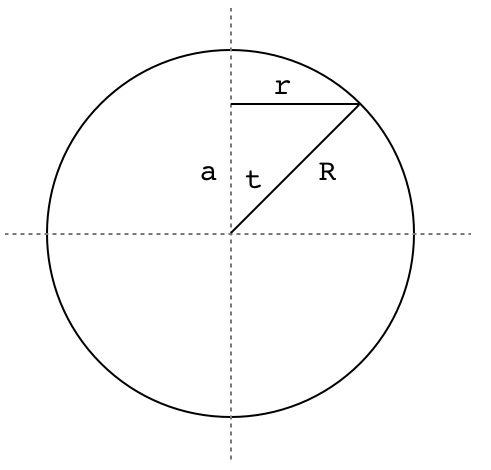
\includegraphics [scale=0.5] {sphere_plane1.png} \end{center}

First of all, we need the coordinates for the intersection of the plane and sphere.  If we imagine a cross-section in the $xz$-plane, we can draw a right triangle with hypotenuse $R$, here equal to $1$, with one of the other sides being the distance from the origin to the plane ($a = 1/\sqrt{2}$), and the third side is the radius of the circle formed when the plane intersects the sphere.

\[ r^2 + a^2 = R^2 \]
\[ r^2 = 1 - (\frac{1}{\sqrt{2}})^2 = \frac{1}{2} = a^2  \]
\[ r = a \]

Solving this reveals that $r = 1/\sqrt{2}$ as well, so this is an isosceles triangle.

Since it's isosceles the tangent of the angle $\phi$ for spherical coordinates (labeled $t$ in the figure) is equal to $1$, so $\phi = \pi/4$ at the edge of the circle of intersection.  The bounds for the integral in spherical coordinates with respect to $\phi$ are $\phi = 0 \rightarrow \pi/4$.

\subsection*{Area of spherical cap}

A bit of a detour, back to the spherical cap, now we know that $r=a$.

We recall that we also found a nice formula for the area of a spherical cap, which is a bit counter-intuitive since it holds also for a spherical belt, and that gives an easy way to remember it

\[ A = 2 \pi R h = 2 \pi (R-a) \]

This leads to a very simple calculation for the volume of the cap.  We find the volume of the whole spherical cone (the volume enclosed by the surface area and all the rays out from the origin tracing its circumference.  It is simply that fraction of the whole surface area, times the volume

\[ V = 2 \pi (R-a) \cdot \frac{4/3 \pi R^3}{4 \pi R^2} \]
\[ = \frac{2}{3} \pi (R^2 - Ra) \]

We must subtract from this the part of the volume (a cone) that lies below the plane

\[ V = \frac{2}{3} \pi (R^2 - Ra) - \frac{1}{3} \pi a^3 \] 
\[ = \frac{2}{3} \pi (R^2 - Ra - \frac{1}{2} a^3) \] 

Plugging in for $R=1$ and $a=1/\sqrt{2}$

\[ = \frac{2}{3} \pi (1 - \frac{1}{\sqrt{2}} - \frac{1}{4 \sqrt{2}}) \] 
\[ = \frac{2}{3} \pi (1 - \frac{5}{4 \sqrt{2}}) \] 

That was easy!

\subsection*{cylindrical coordinates}

We need to decide whether to integrate the region below the plane, or above it.

Let's try above the plane first.  We will integrate with respect to $z$ first.  That means that $r$ is fixed in the inner integral.  The lower bound on $z$ is the height of the plane, $a = 1/\sqrt{2}$.  The upper bound is $\sqrt{R^2 - r^2}$.

So our integral is:

\[ V = \iiint dz \ r \ dr \ d \theta \]
\[ = \int_0^{2\pi} \int_0^a \int_a^{\sqrt{R^2 - r^2}} \ dz \ r \ dr \ d \theta \]

The inner integral is just

\[ \sqrt{R^2 - r^2} -a \]

The middle integral is then

\[ \int_0^a \sqrt{R^2 - r^2} \ r \ dr - a \int_0^a r \ dr \]
\[ = -\frac{1}{3} (R^2 - r^2)^{3/2} - \frac{ar^2}{2} \ \bigg |_0^a \]
\[ = -\frac{1}{3} (R^2 - a^2)^{3/2} - \frac{a^3}{2} + \frac{1}{3} (R^2)^{3/2} \]

This cleans up quite a bit.  First, $R=1$ and $a^2 = 1/2$ so

\[ = -\frac{1}{3} (1 - \frac{1}{2})^{3/2} - \frac{1}{2} \cdot \frac{a}{2} + \frac{1}{3} \]

substitute for the last factor of $a$

\[ = -\frac{1}{3} \cdot \frac{1}{2\sqrt{2}} -\frac{1}{4 \sqrt{2}} +   \frac{1}{3} \]
\[ = \frac{1}{3}(-\frac{1}{2\sqrt{2}} - \frac{3}{4\sqrt{2}} + 1) \]

And finally, we pick up a factor of $2 \pi$ from the outside integral and combine the square root terms at the back of the expression giving

\[ V = \frac{2}{3} \pi (1 - \frac{5}{4 \sqrt{2}}) \]

which is what we had before.

\subsection*{cylindrical coordinates, from below}

We should also be able to do the region below the plane.  In that case we will have a region at the edge of the sphere where the upper bound on $z$ lies on the sphere, whereas in the middle, under the circular intersection with the plane, the upper bound on $z$ is the plane.  

We will have to split the calculation into two parts.  However, the inside part is just a cylinder of radius and height both equal to $a$.

What about the outer ring?  We have $r=a \rightarrow 1$ and $z=0 \rightarrow \sqrt{R^2-r^2}$.

\[ = \int_0^{2\pi} \int_a^1 \int_0^{ \sqrt{R^2-r^2}} \ dz \ r \ dr \ d \theta \]

The inner integral is just $ \sqrt{R^2-r^2}$ so the middle integral is

\[ \int_a^1   \sqrt{R^2-r^2} \ r \ dr \]
\[ = -\frac{1}{3} (R^2 - r^2)^{3/2} \ \bigg |_a^1 \]

Since $R = 1$, this is just

\[ = \frac{1}{3} (1 - a^2)^{3/2} \]

times $2\pi$ for the outer integral gives 

\[ = \frac{2}{3}\pi (1 - a^2)^{3/2} \]

Now, for the cylinder, we have

\[ V = \pi r^2 h \]

Both the height and radius are equal to $a$ so

\[ = \pi a^3 \]

Combined with the outer ring we have

\[ = \frac{2}{3}\pi \ [ \ 1 - a^2)^{3/2} +  \pi a^3\ ] \]

Subtracted from the hemisphere, we obtain

\[= \frac{2}{3} \pi R^3 - \frac{2}{3}\pi (1 - a^2)^{3/2} -  \pi a^3 \]

To evaluate this, factor out the $2 \pi/3$ and recall that $R=1$

\[= \frac{2}{3} \pi  \ [ \ 1 -  (1 - a^2)^{3/2} -  \frac{3}{2} a^2 \cdot a)\ ] \]

Substitute $a^2 = 1/2$

\[= \frac{2}{3} \pi  \ [ \ 1 -  (\frac{1}{2})^{3/2} -  \frac{3}{4} \cdot a)\ ] \]
\[= \frac{2}{3} \pi  \ [ \ 1 -  \frac{1}{2 \sqrt{2}} -  \frac{3}{4} \cdot a)\ ] \]

Finally, substitute  $a = 1/\sqrt{2}$

\[= \frac{2}{3} \pi  \ [ \ 1 -  \frac{5}{4 \sqrt{2}} \ ] \]

\subsection*{spherical coordinates}

Let's do this problem in spherical coordinates, while we're at it.  We will integrate in the same order as usual, first with respect to $\rho$ and next with respect to $\phi$, and then finally with respect to $\theta$.

And again, what we know at this point is simply that the distance from the origin to the plane that begins our region of integration is $1/\sqrt{2}$.  

Let't tackle $\phi$ first.  If we imagine a cross-section in the $xz$-plane, we can draw a right triangle with hypotenuse equal to $R$, here equal to $1$, formed with one side equal to the distance from the origin to the plane ($1/\sqrt{2}$) and the other side just being the radius of the circle formed when the plane intersects the sphere.

\[ r^2 + (\frac{1}{\sqrt{2}})^2 = 1 \]

Solving this, we find that $r = 1/\sqrt{2}$ as well, so this is an isosceles triangle.  Therefore the tangent of $\phi$ is equal to one, and so $\phi = \pi/4$.  The bounds for the integral with respect to $\phi$ are $\phi = 0 \rightarrow \pi/4$.

The second question is the bounds on $\rho$.  Remember, for the inner integral we have $\phi$ \emph{fixed}.  Using the same cross-section with the $xz$-axis, we find that the part of the ray along the radius that lies inside the volume we don't want, times the cosine of $\phi$, is equal to the height.

\begin{center} 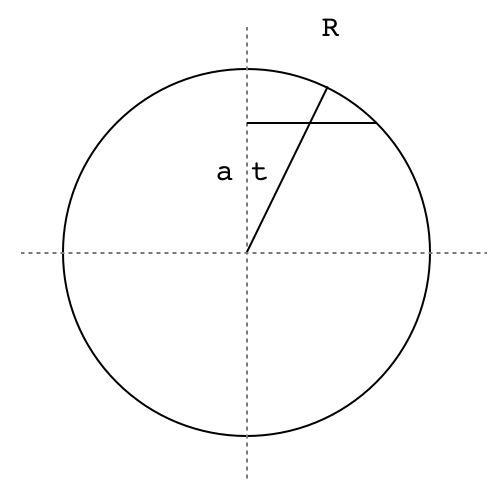
\includegraphics [scale=0.5] {sphere_plane2.png} \end{center}

\[ \rho_{start} \cos \phi = \frac{1}{\sqrt{2}} \]
\[ \rho_{start} = \frac{1}{\sqrt{2} \cos \phi} \]

So our triple integral is 

\[ \iiint \rho^2 \sin \phi \ d \rho \ d \phi \ d \theta \]
\[ = \int_{\theta = 0}^{2 \pi} \int_{\phi=0}^{\pi/4} \int_{\rho = 1/\sqrt{2} \cos \phi}^{R} \rho^2 \sin \phi \ d \rho \ d \phi \ d \theta \]

For the inner integral we have 

\[ \sin \phi \ \frac{\rho^3}{3} \ \bigg  |_{1/\sqrt{2} \cos \phi}^{R} \]
\[ = \frac{1}{3} \sin \phi (R^3 - \frac{1}{2 \sqrt{2} \cos^3 \phi}) \]

For the middle integral we need to integrate with respect to $\phi$.  The first part is just

\[ \int \sin \phi \ d \phi = - \cos \phi \]

The second term is 

\[ \int \tan \phi \sec^2 \phi \ d \phi = \frac{1}{2} \tan^2 \phi \]

Hold aside the factor of $1/3$ for a moment.  We have two terms from the integral

\[ -R^3 \cos \phi \ \bigg  |_{0}^{\pi/4} \]
\[ -\frac{1}{4 \sqrt{2}}\ \tan^2 \phi \ \bigg  |_{0}^{\pi/4} \]

The first term evaluates to

\[ -R^3 (\frac{1}{\sqrt{2}} - 1) = (1- \frac{1}{\sqrt{2}})R^3 \]

And the second is just

\[ -\frac{1}{4 \sqrt{2}} \]

Putting it all together we obtain:

\[ \frac{1}{3} \ [ \ (1- \frac{1}{\sqrt{2}})R^3 - \frac{1}{4 \sqrt{2}} \ ] \]

Of course, $R=1$ so

\[ = \frac{1}{3} \ [ \ 1- \frac{1}{\sqrt{2}} - \frac{1}{4 \sqrt{2}} \ ] \]
\[ = \frac{1}{3} \ [ \ 1-  \frac{5}{4 \sqrt{2}} \ ] \]

All times $2 \pi$

\[ = \frac{2}{3}\pi \ [ \ 1-  \frac{5}{4 \sqrt{2}} \ ] \]

And that looks the same as every other calculation.

\subsection*{spherical coordinates, bottom section}

At first I set up this integral, which is correct so far as it goes, but in the process we miss the region under the plane where $\phi=0 \rightarrow \pi/4$ (we'll come back for it).  This part is a "tire" with triangular cross-section.

\[ = \int_{\theta = 0}^{2 \pi} \int_{\phi=\pi/4}^{\pi/2} \int_{\rho=0}^{R} \rho^2 \sin \phi \ d \rho \ d \phi \ d \theta \]

\[ = \frac{1}{3} \int_{\phi=\pi/4}^{\pi/2} \ \sin \phi \ d \phi \]
\[ = -\frac{1}{3} \cos \phi \ \bigg |_{\pi/4}^{\pi/2} \]
\[ = (-\frac{1}{3}) (0- \frac{1}{\sqrt{2}}) \]
\[ = \frac{1}{3 \sqrt{2}} \]

Times $2\pi$ gives

\[ = \frac{2}{3}\pi (\frac{1}{ \sqrt{2}}) \]

We must subtract that from the hemisphere, obtaining

\[ = \frac{2}{3}\pi (1 - \frac{1}{ \sqrt{2}}) \]

The additional region we need to subtract is the region where $\phi=0 \rightarrow \pi/4$.  This is a cone (under the plane) of height and radius $a$ and volume

\[ \frac{1}{3} \pi a^3 \]
\[ =  \frac{1}{3} \pi (\frac{1}{2 \sqrt{2}}) \]
\[ =  \frac{2}{3} \pi (\frac{1}{4 \sqrt{2}}) \]

Once we subtract that, our answer matches every other answer in this write-up.

\[ = \frac{2}{3}\pi (1 - \frac{1}{ \sqrt{2}} - \frac{1}{4 \sqrt{2}}) \]
\[ = \frac{2}{3}\pi (1 - \frac{5}{4 \sqrt{2}}) \]

And having done that, we see how all the areas relate to one another.  Leaving aside the factor of $2 \pi/3$, we have 

the hemisphere ($1$)

the triangular "tire" shape ($1/\sqrt{2}$)

the cone under the plane ($1/4\sqrt{2}$)

the cylinder($3/4\sqrt{2}$)

the outer ring($1/2 \sqrt{2}$)

and the spherical cap($1 - 5/4 \sqrt{2}$), which is hemisphere minus (tire plus cone) or hemisphere minus (cylinder plus ring).


\end{document}  